\setcounter{ExampleCounter}{1}
Once we can talk about individual sets, we can start thinking about relationships among these sets.  For instance, think back to the example from the chapter introduction about a library categorizing books in their collection.

If they have a set of books written in the 20th century, and they have a set of science fiction books, we could ``combine'' these two sets and look for only the science fiction novels written in the 20th century, excluding other books written in the 20th century and other science fiction.

On the other hand, we could look for any book written in the 20th century that is NOT in the category of science fiction.  And of course there are other combinations we could make with these two sets.

This is similar to the way we can use a search engine like Google to refine the results of a search.\footnote{See the first section of the chapter on Logic for more details.}\\

We'll define four operations that we can use to describe the relationship between two sets:
\begin{enumerate}
\item The \textbf{complement} of a set
\item The \textbf{union} of two sets
\item The \textbf{intersection} of two sets
\item The \textbf{difference} between two sets
\end{enumerate}

You'll find that these operations are well named, because their names describe what they do.\\

Before we get to those, though, we need to define what we call the \textbf{universal set}, because we'll need to keep track of this universal set when we look at examples.

\begin{formula}{Universal Set}
In a particular situation,\footnote{The universal set will be different in different problems.} the \textbf{universal set} is the set of all the objects that we are considering in this context.
\end{formula}

In other words, if the problems starts by describing the books in a library, then the set of all the books at that library will be the universal set.  On the other hand, if the problem starts with the students in your classroom, those students will form the universal set.

\subsection{Venn Diagrams}
As we go through these operations, it will be helpful to use diagrams to visualize them; these diagrams are called \textbf{Venn diagrams}, since they were introduced by John Venn in 1880.  A basic Venn diagram consists of a box (usually shown) that represents the universal set, and circles inside that box that represent sets that we want to talk about.

\begin{center}
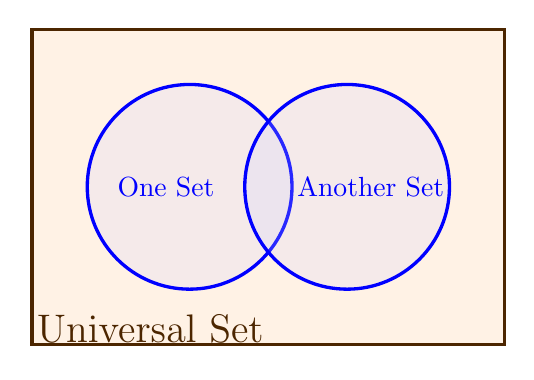
\begin{tikzpicture}
  \draw [very thick,color=orange!30!black, fill=orange, fill opacity=0.1] (-3cm,-2cm) rectangle (3cm,2cm);

  \draw [very thick,color=blue, fill=blue!20, fill opacity=0.2] (-1,0) circle (1.3cm);
  \draw [very thick,color=blue, fill=blue!20, fill opacity=0.2] (1,0) circle (1.3cm);
  \draw [yshift=0cm,xshift=-1.3cm] node {\color{blue} One Set};
  \draw [yshift=0cm,xshift=1.3cm] node {\color{blue} Another Set};
  
  %\draw [very thick,color=blue, fill=blue!20] (0.8,0) circle (1.2cm);
  %\draw [yshift=1.8cm,xshift=0.8cm] node {\color{blue}\Large Fiction};
  
  %\draw [yshift=-3cm,xshift=1.5cm] node (a) {\color{orange!40!black}\Large NOT Fiction};
  %\draw [yshift=-1cm,xshift=2cm] node (b) {};
  \draw [yshift=-1.8cm,xshift=-1.5cm] node {\color{orange!30!black}\Large Universal Set};
  
  %\draw [ultra thick,color=blue!50!red, fill=blue!50!red] (0,-0.9) arc (-45:45:1.28cm);
  %\draw [ultra thick,color=blue!50!red, fill=blue!50!red] (-0.03,0.89) arc (135:225:1.24cm);
  %\draw [ultra thick,color=blue!50!red] (0,-0.9) -- (0,0.9);
  
  %\draw [ultra thick] (a) -- (b);
\end{tikzpicture}
\end{center}

Notice the overlapping region in the middle; this represents the elements that belong to both sets.
\vfill
\pagebreak

For instance, we could categorize students in your classroom by hair color and eye color, specifically looking at the set of students who have brown hair and the set of students with brown eyes.

\begin{center}
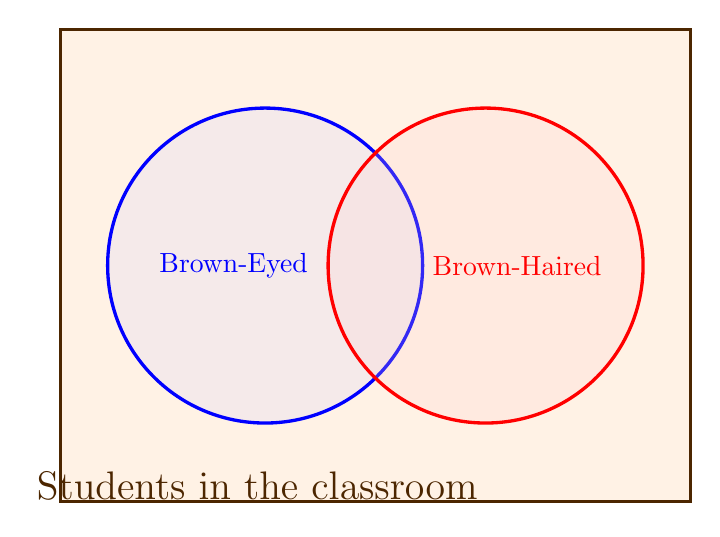
\begin{tikzpicture}
  \draw [very thick,color=orange!30!black, fill=orange, fill opacity=0.1] (-4cm,-3cm) rectangle (4cm,3cm);

  \draw [very thick,color=blue, fill=blue!20, fill opacity=0.2] (-1.4,0) circle (2cm);
  \draw [very thick,color=red, fill=red!20, fill opacity=0.2] (1.4,0) circle (2cm);
  \draw [yshift=0cm,xshift=-1.8cm] node {\color{blue} Brown-Eyed};
  \draw [yshift=0cm,xshift=1.8cm] node {\color{red} Brown-Haired};
  
  \draw [yshift=-2.8cm,xshift=-1.5cm] node {\color{orange!30!black}\Large Students in the classroom};
  
\end{tikzpicture}
\end{center}

There are (probably) some students in the overlapping region, who have brown hair and brown eyes.  But it is certainly possible to have brown eyes and not brown hair, and vice versa.  Also, it is possible to not have brown eyes or brown hair, and these would be the students inside the rectangle but outside of both circles.\\

We could have an example, though, where there are no shared elements between the two sets.  For instance, if the two sets we considered were ``letters in the Greek alphabet'' and ``letters in the Hebrew alphabet,'' those two circles would not overlap at all.  We call these \textbf{disjoint sets}.

\begin{center}
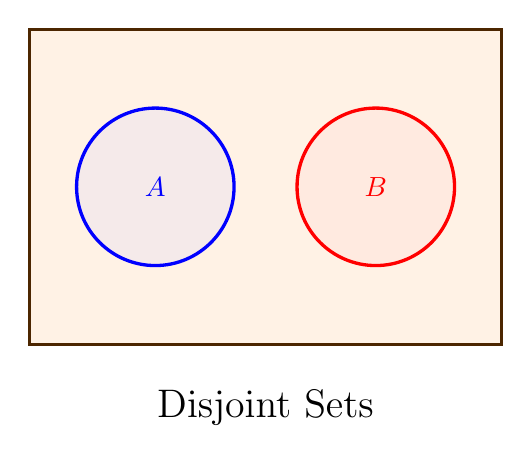
\begin{tikzpicture}
  \draw [very thick,color=orange!30!black, fill=orange, fill opacity=0.1] (-3cm,-2cm) rectangle (3cm,2cm);

  \draw [very thick,color=blue, fill=blue!20, fill opacity=0.2] (-1.4,0) circle (1cm);
  \draw [very thick,color=red, fill=red!20, fill opacity=0.2] (1.4,0) circle (1cm);
  \draw [yshift=0cm,xshift=-1.4cm] node {\color{blue} $A$};
  \draw [yshift=0cm,xshift=1.4cm] node {\color{red} $B$};
  
  \draw [yshift=-2.8cm,xshift=0cm] node {\Large Disjoint Sets};
  
\end{tikzpicture}
\end{center}

We could also have an example where one set is completely contained in another, like in the case of the sets ``all students'' and ``students at your school.''

\begin{center}
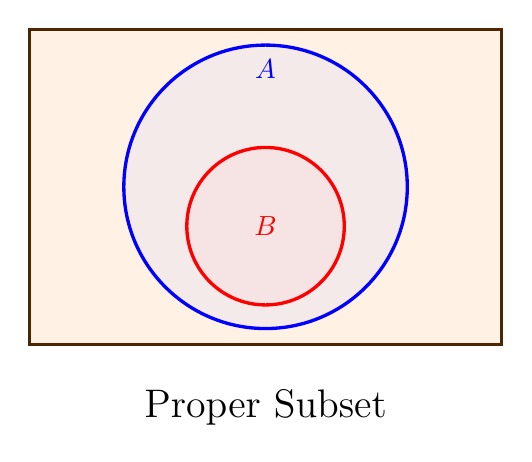
\begin{tikzpicture}
  \draw [very thick,color=orange!30!black, fill=orange, fill opacity=0.1] (-3cm,-2cm) rectangle (3cm,2cm);

  \draw [very thick,color=blue, fill=blue!20, fill opacity=0.2] (0,0) circle (1.8cm);
  \draw [very thick,color=red, fill=red!20, fill opacity=0.2] (0,-0.5) circle (1cm);
  \draw [yshift=1.5cm,xshift=0cm] node {\color{blue} $A$};
  \draw [yshift=-0.5cm,xshift=0cm] node {\color{red} $B$};
  
  \draw [yshift=-2.8cm,xshift=0cm] node {\Large Proper Subset};
  
\end{tikzpicture}
\end{center}

Now that we have Venn diagrams at our disposal, we're ready to define the complement, union, intersection, and difference.
\vfill
\pagebreak

\subsection{Complement}
\begin{formula}{Complement}
The \textbf{complement} of a set $A$, denoted\footnote{Other books might write $A'$ or $\overline{A}$ to indicate the complement.} $A^c$ consists of all elements (in the universal set) that \textbf{do not} belong to $A$.

\begin{center}
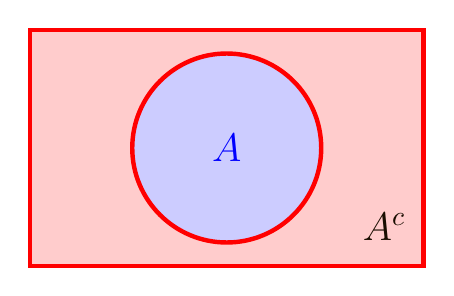
\begin{tikzpicture}
  \draw [ultra thick,color=red, fill=red!20] (-2.5cm,-1.5cm) rectangle (2.5cm,1.5cm);

  \draw [ultra thick,color=red, fill=blue!20] (0,0) circle (1.2cm);
  \draw [yshift=0cm,xshift=0cm] node {\color{blue}\Large $A$};
  
  %\draw [very thick,color=blue, fill=blue!20] (0.8,0) circle (1.2cm);
  %\draw [yshift=1.8cm,xshift=0.8cm] node {\color{blue}\Large Fiction};
  
  \draw [yshift=-1cm,xshift=2cm] node (a) {\color{orange!10!black}\Large $A^c$};
  %\draw [yshift=-1cm,xshift=2cm] node (b) {};
  
  
  %\draw [ultra thick,color=blue!50!red, fill=blue!50!red] (0,-0.9) arc (-45:45:1.28cm);
  %\draw [ultra thick,color=blue!50!red, fill=blue!50!red] (-0.03,0.89) arc (135:225:1.24cm);
  %\draw [ultra thick,color=blue!50!red] (0,-0.9) -- (0,0.9);
  
  %\draw [ultra thick] (a) -- (b);
\end{tikzpicture}
\end{center}

\[A^c = \{x\ |\ x \in U \textrm{ and } x \notin A\}\]
\end{formula}

\begin{example}{Complement}
In the alphabet, find the complement of $V$, the set of vowels.

\sol
The complement of the vowels (i.e. the letters that aren't vowels) is the set of consonants:\marginnote{We're assuming that y is not a vowel}
\[\boxed{V^c = \{b,c,d,f,g,h,j,k,l,m,n,p,q,r,s,t,v,w,x,y,z\}}\]

Notice that we especially need a well defined universal set (like the 26 letters of the alphabet) to be able to describe the complement of a set clearly.
\end{example}

\begin{example}{Complement}
Given the universal set $U = \mathbb{N}$, find the complement of \[A = \{x \in \mathbb{N}\ |\ x \geq 10\}.\]

\sol
The complement of the natural numbers greater than or equal to 10 is, as you may expect, the natural numbers less than 10 (notice that 10 is in $A$, so it is not in $A^c$):
\[\boxed{A^c = \{x \in \mathbb{N}\ |\ x < 10\} = \{1,2,3,4,5,6,7,8,9\}}\]
\end{example}

\begin{example}{Complement}
If the universe is $U = \{1,2,3,\ldots,10\}$, find the complement of the set $E=\varnothing$.

\sol
The complement of the empty set is the set of all points in the universe:
\[\boxed{E^c = U = \{1,2,3,\ldots,10\}}\]
\end{example}
\pagebreak

\subsection{Union}
\begin{formula}{Union}
The \textbf{union} of two sets $A$ and $B$, denoted\footnote{You can remember this because the symbol looks like a U for union.} $A \cup B$, consists of all elements that are \textbf{either in $A$ or in $B$ OR BOTH}.\marginnote{This is the part that trips up the most people.  The union includes elements that are in both sets, which isn't necessarily how we tend to use the word ``or''; for instance, if someone said ``write down your first name or your last name,'' you wouldn't think to write both.  The way we often use it in English is called the \emph{exclusive} OR, meaning that it doesn't include ``...or both,'' but in set theory (and logic) we use the \emph{inclusive} OR.}

\begin{center}
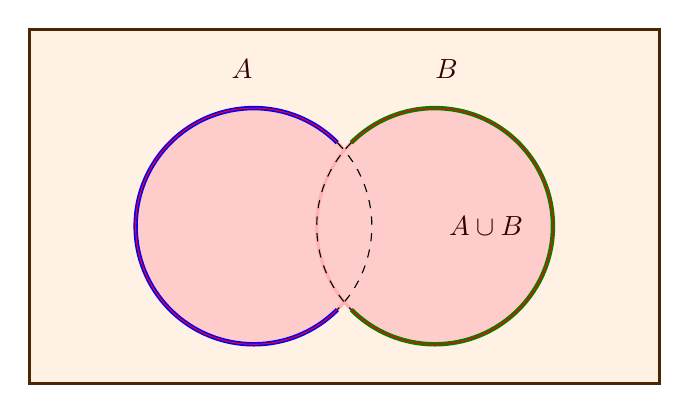
\begin{tikzpicture}
  \draw [very thick,color=orange!30!black, fill=orange, fill opacity=0.1] (-4cm,-2cm) rectangle (4cm,2.5cm);

  \draw [very thick,color=red!30, fill=red!20] (-1.15,0) circle (1.5cm);
  \draw [very thick,color=red!30, fill=red!20] (1.15,0) circle (1.5cm);
  \draw [yshift=2cm,xshift=-1.3cm] node {\color{red!20!black} $A$};
  \draw [yshift=2cm,xshift=1.3cm] node {\color{red!20!black} $B$};
  
  \draw [yshift=0cm,xshift=1.8cm] node {\color{red!20!black} $A \cup B$};
  
  \draw [ultra thick, color=blue] (-1.15,0) ++(45:1.5) arc (45:315:1.5);
  \draw [ultra thick, color=green!50!black] (1.15,0) ++(135:1.5) arc (135:-135:1.5);
  \draw [color=red] (-1.15,0) ++(45:1.5) arc (45:315:1.5);
  \draw [color=red] (1.15,0) ++(135:1.5) arc (135:-135:1.5);
  
  \draw [dashed,color=black] (-1.15,0) ++(45:1.5) arc (45:-45:1.5);
  \draw [dashed,color=black] (1.15,0) ++(135:1.5) arc (135:225:1.5);
  
\end{tikzpicture}
\end{center}
\[A \cup B = \{x\ |\ x \in A \textrm{ or } x \in B\}\]
\end{formula}

Again, note that all it takes for an element to be in the union of two sets is for it to belong to \emph{at least} one of them.  For instance, you'd be in the union of ``people who own a car'' and ``people who own a bike'' as long as you owned \emph{at least} one of those; if you owned a car \emph{and} a bike, you'd also be in the union.

\begin{example}{Union}
Find the union of the following sets.
\begin{enumerate}[(a)]
\item $A = \{5,6,2,4\} \ \ \textrm{ and } \ \ B = \{1,4\}$
\item $A = \{a,b,c,d\} \ \ \textrm{ and } \ \ B = \{x,y,z\}$
\item $A = \mathbb{N} \ \ \textrm{ and } \ \ B = \varnothing$
\end{enumerate}

\sol
\begin{enumerate}[(a)]
\item Again, the union of two sets is all the elements that are in either set (we only list repeated elements once):
\[\boxed{A \cup B = \{5,6,2,4,1\}}\]  Remember, the order in which we list the elements in a set is not significant.

\item Here there are no elements common to both sets:
\[\boxed{A \cup B = \{a, b, c, d, x, y, z\}}\]

\item Note that if you take the union of any set with the empty set, you'll get the set you started with, because the empty set doesn't add anything:
\[\boxed{A \cup B = \mathbb{N} \cup \varnothing = \mathbb{N}}\]
\end{enumerate}
\end{example}

\begin{try}[http://hartleymath.com/versatilemath/tryit/\#/set-theory--set-union]
If $A=\{1,3,5,7\}$ and $B=\{2,3,4\}$, find $A \cup B$.
\end{try}
\vfill
\pagebreak

\subsection{Intersection}
\begin{formula}{Intersection}
The \textbf{intersection} of two sets $A$ and $B$, denoted $A \cap B$, consists of all elements that are \textbf{in both $A$ and $B$}.

\begin{center}
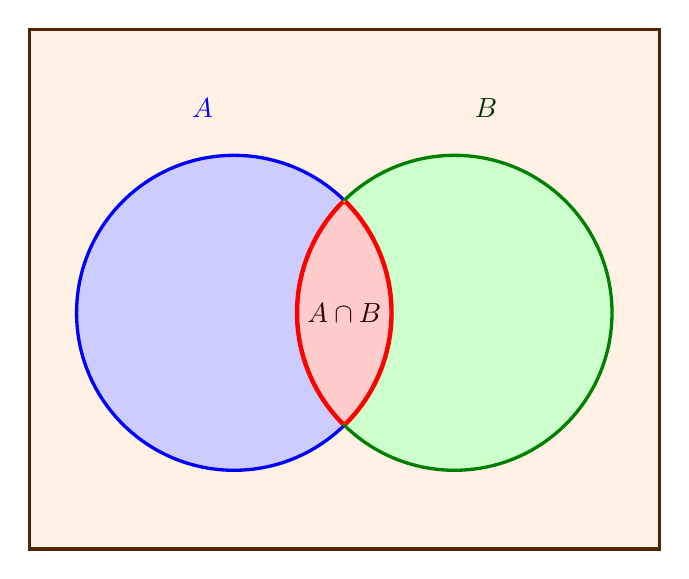
\begin{tikzpicture}
  \draw [very thick,color=orange!30!black, fill=orange, fill opacity=0.1] (-4cm,-3cm) rectangle (4cm,3.6cm);

  \draw [very thick,color=blue, fill=blue!20] (-1.4,0) circle (2cm);
  \draw [very thick,color=green!50!black, fill=green!20] (1.4,0) circle (2cm);
  \draw [yshift=2.6cm,xshift=-1.8cm] node {\color{blue} $A$};
  \draw [yshift=2.6cm,xshift=1.8cm] node {\color{green!20!black} $B$};
  
  
  
  %\draw [ultra thick, color=red] (-1.4,0) ++(45:2) arc (45:315:2);
  %\draw [ultra thick, color=red] (1.4,0) ++(135:2) arc (135:-135:2);
  
  \draw [ultra thick,color=red!20] (0,-1.414) -- (0,1.414);
  \draw [ultra thick,color=red,fill=red!20] (-1.4,0) ++(45:2) arc (45:-45:2);
  \draw [ultra thick,color=red,fill=red!20] (1.4,0) ++(135:2) arc (135:225:2);
  \draw [yshift=0cm,xshift=0cm] node {\color{red!20!black} $A \cap B$};
  
\end{tikzpicture}
\end{center}
\[A \cap B = \{x\ |\ x \in A \textrm{ and } x \in B\}\]
\vspace{0.1in}
\end{formula}

\begin{example}{Intersection}
Find the intersection of each pair of sets.

\begin{enumerate}[(a)]
\item $\{1,3,5,7,9\} \cap \{2,3,4,5\}$
\item $\{x\ |\ x \textrm{ is even}\} \cap \{x\ |\ x \textrm{ is odd}\}$
\item $\mathbb{N} \cap \varnothing$
\end{enumerate}

\sol
\begin{enumerate}[(a)]
\item $\{1,3,5,7,9\} \cap \{2,3,4,5\} = \boxed{\{3,5\}}$
\item $\{x\ |\ x \textrm{ is even}\} \cap \{x\ |\ x \textrm{ is odd}\} = \boxed{\varnothing}$
\item $\mathbb{N} \cap \varnothing = \boxed{\varnothing}$
\end{enumerate}
\end{example}

\begin{try}[http://hartleymath.com/versatilemath/tryit/\#/set-theory--set-intersection]
If $A=\{1,3,5,7\}$ and $B=\{2,3,4\}$, find $A \cap B$.
\end{try}

\paragraph{Note:} look back at that last example and make sure you can verify that for any set $A$, 
\begin{align*}
A &\cup \varnothing = A\\
A &\cap \varnothing = \varnothing
\end{align*}
\pagebreak

\subsection{Difference}
The difference between two sets is fairly intuitive: it consists of all the elements of the first set that are \textbf{not} elements of the second set.  In other words, take the first set and \emph{remove} any elements from it that also show up in the second set, and what's left is the difference.\\

The only unusual part is the symbol we use to denote this; it looks like a minus sign, but it's slanted to indicate that we're finding a \emph{set} difference, not the difference between two numbers.

\begin{formula}{Difference}
The \textbf{difference} of two sets $A$ and $B$, denoted $A \setminus B$, consists of all elements that are \textbf{in $A$, but not in $B$}.

\begin{center}
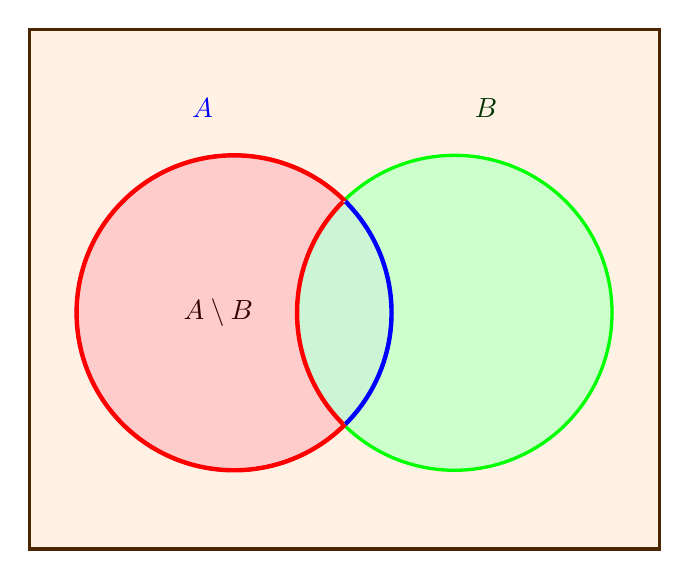
\begin{tikzpicture}
  \draw [very thick,color=orange!30!black, fill=orange, fill opacity=0.1] (-4cm,-3cm) rectangle (4cm,3.6cm);

  \draw [very thick,color=blue, fill=red!20] (-1.4,0) circle (2cm);
  \draw [very thick,color=green, fill=green!20] (1.4,0) circle (2cm);
  \draw [yshift=2.6cm,xshift=-1.8cm] node {\color{blue} $A$};
  \draw [yshift=2.6cm,xshift=1.8cm] node {\color{green!20!black} $B$};
  
  
  
  \draw [ultra thick, color=red] (-1.4,0) ++(45:2) arc (45:315:2);
  %\draw [ultra thick, color=red] (1.4,0) ++(135:2) arc (135:-135:2);
  
  \draw [ultra thick,color=blue!20!green!20] (0,-1.414) -- (0,1.414);
  \draw [ultra thick,color=blue,fill=blue!20!green!20] (-1.4,0) ++(45:2) arc (45:-45:2);
  \draw [ultra thick,color=red,fill=blue!20!green!20] (1.4,0) ++(135:2) arc (135:225:2);
  \draw [yshift=0cm,xshift=-1.6cm] node {\color{red!20!black} $A \setminus B$};
  
\end{tikzpicture}
\end{center}
\[A \setminus B = \{x\ |\ x \in A \textrm{ and } x \notin B\}\]
\vspace{0.1in}
\end{formula}

\begin{example}{Difference}
If $A$ consist of whole numbers from 1 to 9, and $B = \{7,8,9,10,\ldots\}$, find $A \setminus B$.

\sol
Take away every element from $A$ that also occurs in $B$, and you get
\[\boxed{A \setminus B = \{1,2,3,4,5,6\}}\]
\end{example}

\begin{try}[http://hartleymath.com/versatilemath/tryit/\#/set-theory--set-difference]
If $A=\{1,3,5,7\}$ and $B=\{2,3,4\}$, find $A \setminus B$.
\end{try}

\paragraph{Note:} Since the difference is everything that is in $A$ AND (intersection) NOT (complement) in $B$, we can write the difference in terms of the intersection and complement:
\[A \setminus B = A \cap B^c\]
\pagebreak

\begin{example}{Difference}
Use the following sets to illustrate that \[A \setminus B = A \cap B^c.\]

\begin{align*}
A &= \{1,2,3,4,5,6,7,8,9\}\\
B &= \{7,8,9,10,\ldots\}
\end{align*}

\sol
We just found the difference $A \setminus B$ in the last example:
\[A \setminus B = \{1,2,3,4,5,6\}\]

Now we just have to show that if we find $A \cap B^c$, we get the same answer:
\[B^c = \{\ldots, 4,5,6\} \longrightarrow A \cap B^c = \{1,2,3,4,5,6\}\]

\end{example}

\subsection{Combining Operations}
As we just saw with $A \cap B^c$, we can use several set operations in combination.  If we need to, we can use parentheses as grouping symbols to make the order of operations clear.

\begin{example}{Combining Operations}
Suppose that $U = \{1,2,3,4,5,6,7,8,9,10\}$, $A=\{1,3,5,7\}$, and $B=\{4,5,6,7\}$.  Find each of the following.
\begin{enumerate}[(a)]
\item $(A \cup B)^c$
\item $A^c \cap B^c$
\item $(A \cap B)^c$
\item $A^c \cup B^c$
\end{enumerate}

\sol
\begin{enumerate}[(a)]
\item Note that according to the parentheses, we need to start by finding $A \cup B$, and then we need to take the complement of this union:
\begin{align*}
A \cup B &= \{1,3,4,5,6,7\}\\
&\implies \boxed{(A \cup B)^c = \{2,8,9,10\}}
\end{align*}

\item Since there are no parentheses, we'll first find the two complements individually, and then find their intersection:
\begin{align*}
A^c &= \{2,4,6,8,9,10\} \ \ \textrm{ and } \ \ B^c = \{1,2,3,8,9,10\}\\
&\implies \boxed{A^c \cap B^c = \{2,8,9,10\}}
\end{align*}

\item Here again we start inside the parentheses:
\begin{align*}
A \cap B &= \{5,7\}\\
&\implies \boxed{(A \cap B)^c = \{1,2,3,4,6,8,9,10\}}
\end{align*}

\item Finally, take the union of the complements:
\begin{align*}
A^c &= \{2,4,6,8,9,10\} \ \ \textrm{ and } \ \ B^c = \{1,2,3,8,9,10\}\\
&\implies \boxed{A^c \cup B^c = \{1,2,3,4,6,8,9,10\}}
\end{align*}
\end{enumerate}
\end{example}

\begin{try}[http://hartleymath.com/versatilemath/tryit/\#/set-theory--combining-set-operations-numbers]
For the sets listed in the example above, find
\begin{enumerate}[(a)]
\item $A^c \cup B$
\item $A \cap B^c$
\item $B \cup B^c$
\item $A \cap A^c$
\end{enumerate}
\end{try}

Notice something interesting: that example, as a side note, illustrates the following two facts:
\begin{align*}
(A \cup B)^c &= A^c \cap B^c\\
(A \cap B)^c &= A^c \cup B^c
\end{align*}

These are known as \textbf{De Morgan's laws}, and we'll restate and explain them in the next section, but before you get there, see if you can come up with an intuitive way of explaining why this makes sense.  Maybe think of some simple, well-defined sets, and see if you can understand why the complement of the union is the intersection of the complements, and vice versa.\\

It may also help to draw some Venn diagrams to visualize this.

\subsection{Using Three Sets}

Extending the use of set operations to three sets (or more) is not difficult, as long as we're careful, especially with grouping.

\begin{example}{Set Operations with Three Sets}
Suppose that $H=\{$cat, dog, rabbit, mouse$\}$, $F=\{$dog, cow, duck, pig, rabbit$\}$, and $W=\{$duck, rabbit, deer, frog, mouse$\}$.
\begin{enumerate}[(a)]
\item Find $(H \cap F) \cup W$.
\item Find $(H \cap F)^c \cap W$.
\end{enumerate}

\sol
\begin{enumerate}[(a)]
\item Start by finding the intersection: $H \cap F = \{$dog, rabbit$\}$

Then take the union of this answer with $W$:
\[\boxed{(H \cap F) \cup W = \{\textrm{dog, duck, rabbit, deer, frog, mouse}\}}\]

\item We already found this intersection: $H \cap F = \{$dog, rabbit$\}$

Now we want elements that are NOT in this set, and ARE in $W$:
\[\boxed{(H \cap F)^c \cap W = \{\textrm{duck, deer, frog, mouse}\}}\]
\end{enumerate}
\end{example}

\begin{try}[http://hartleymath.com/versatilemath/tryit/\#/set-theory--combining-set-operations-words]
For the sets listed in the example above, find
\begin{enumerate}[(a)]
\item $H \cup F^c \cup W$
\item $H \cap (F \cup W)$
\item $H^c \cap F \cap W$
\end{enumerate}
\end{try}
\vspace{0.3in}

If you want a bit of a challenge, try drawing a Venn diagram for the set $(H \cap F)^c \cap W$.

\begin{formula}{Summary of Set Operations}
\paragraph{Complement:} $A^c = \{x \ |\ x \in U \textrm{ and } x \notin A\}$
\paragraph{Union:} $A \cup B = \{x \ |\ x \in A \textrm{ or } x \in B\}$
\paragraph{Intersection:} $A \cap B = \{x \ |\ x \in A \textrm{ and } x \in B\}$
\paragraph{Difference:} $A \setminus B = \{x \ |\ x \in A \textrm{ and } x \notin B\} = A \cap B^c$
\end{formula}